%-----------------------------------------------------------------------------
% Template for seminar 'Program Analysis' at TU Darmstadt.
%
% Adapted from template for sigplanconf LaTeX Class, which is a LaTeX 2e
% class file for SIGPLAN conference proceedings (by Paul C.
% Anagnostopoulos).
%
%-----------------------------------------------------------------------------


\documentclass[authoryear,preprint]{sigplanconf}
%Define the listing package
\usepackage{listings} %code highlighter
\usepackage{color} %use color
\definecolor{mygreen}{rgb}{0,0.6,0}
\definecolor{mygray}{rgb}{0.5,0.5,0.5}
\definecolor{mymauve}{rgb}{0.58,0,0.82}
 
%Customize a bit the look
\lstset{ %
backgroundcolor=\color{white}, % choose the background color; you must add \usepackage{color} or \usepackage{xcolor}
basicstyle=\footnotesize, % the size of the fonts that are used for the code
breakatwhitespace=false, % sets if automatic breaks should only happen at whitespace
breaklines=true, % sets automatic line breaking
captionpos=b, % sets the caption-position to bottom
commentstyle=\color{mygreen}, % comment style
deletekeywords={...}, % if you want to delete keywords from the given language
escapeinside={\%*}{*)}, % if you want to add LaTeX within your code
extendedchars=true, % lets you use non-ASCII characters; for 8-bits encodings only, does not work with UTF-8
frame=single, % adds a frame around the code
keepspaces=true, % keeps spaces in text, useful for keeping indentation of code (possibly needs columns=flexible)
keywordstyle=\color{blue}, % keyword style
% language=Octave, % the language of the code
morekeywords={*,...}, % if you want to add more keywords to the set
numbers=left, % where to put the line-numbers; possible values are (none, left, right)
numbersep=5pt, % how far the line-numbers are from the code
numberstyle=\tiny\color{mygray}, % the style that is used for the line-numbers
rulecolor=\color{black}, % if not set, the frame-color may be changed on line-breaks within not-black text (e.g. comments (green here))
showspaces=false, % show spaces everywhere adding particular underscores; it overrides 'showstringspaces'
showstringspaces=false, % underline spaces within strings only
showtabs=false, % show tabs within strings adding particular underscores
stepnumber=1, % the step between two line-numbers. If it's 1, each line will be numbered
stringstyle=\color{mymauve}, % string literal style
tabsize=2, % sets default tabsize to 2 spaces
title=\lstname % show the filename of files included with \lstinputlisting; also try caption instead of title
}
%END of listing package%
 
\definecolor{darkgray}{rgb}{.4,.4,.4}
\definecolor{purple}{rgb}{0.65, 0.12, 0.82}
 
%define Javascript language
\lstdefinelanguage{JavaScript}{
keywords={typeof, new, true, false, catch, function, return, null, catch, switch, var, if, in, while, do, else, case, break},
keywordstyle=\color{blue}\bfseries,
ndkeywords={class, export, boolean, throw, implements, import, this},
ndkeywordstyle=\color{darkgray}\bfseries,
identifierstyle=\color{black},
sensitive=false,
comment=[l]{//},
morecomment=[s]{/*}{*/},
commentstyle=\color{purple}\ttfamily,
stringstyle=\color{red}\ttfamily,
morestring=[b]',
morestring=[b]"
}
 
\lstset{
language=JavaScript,
extendedchars=true,
basicstyle=\footnotesize\ttfamily,
showstringspaces=false,
showspaces=false,
numbers=left,
numberstyle=\footnotesize,
numbersep=9pt,
tabsize=2,
breaklines=true,
showtabs=false,
captionpos=b
}

% A couple of packages that may be useful
\usepackage{amsmath}
\usepackage{amsfonts}
\usepackage{amssymb}
\usepackage{amsthm}
\usepackage{algorithm2e}
\usepackage{listings}
\usepackage{xcolor}
\usepackage{tikz}
\usepackage{booktabs}
\usepackage{subfigure}
\usepackage[english]{babel}
\usepackage{blindtext}
\usepackage[T1]{fontenc}
\usepackage{graphicx}
\usepackage{float}
\usepackage{scrextend}
\usepackage{csquotes}
\usepackage{textcomp}

\begin{document}

\special{papersize=a4}
\setlength{\pdfpageheight}{\paperheight}
\setlength{\pdfpagewidth}{\paperwidth}


\title{Hoisting Nested Functions}

\authorinfo{Anam Dodhy}
           {Informatik, TU Darmstadt}
           {anam.dodhy@stud.tu-darmstadt.de}
\authorinfo{Chaitra Hegde}
           {Informatik, TU Darmstadt}
           {chaitra.hegde@stud.tu-darmstadt.de}

\maketitle

\begin{abstract}
With the widespread use of Javascript in web development, performance is a factor of concern which may affect the speed of the browser. One such performance limiting factor is nested functions in JavaScript. In this project, we have developed an analysis using Jalangi2 [Ref:: Jalangi] framework and NodeJS to detect the hoistability of the nested functions in Javascript. This approach is evaluated on the Javascript Library \textit{Lodash}, to check the improvement in the performance of Javascript in Google V8 engines after hoisting nested functions.

\end{abstract}



\section{Introduction}
\label{sec:introduction}
JavaScript is used for both client and server side scripting. Among the many features it provides, one of the features that we are interested in is hoisting of function declarations. \textit{Hoisting} is moving the variables or function declarations outside of the scope they are currently residing in. JavaScript also allows nesting one function inside the other. This is because nesting reduces the global name-space pollution[Ref:: 1]. Also, if a function has to access the local variable of another function then it has to be nested under the function whose variable it wants to access. This helps in maintaining the privacy of data inside the function. \par

The nested (inner) function is created only when the parent (outer) function is invoked. So if the outer function is called in a loop then the nested function gets created on every single call no matter if it is used for the computation or not. This would reduce the performance of the Javascript engine. So if the nested functions are not dependent on any variables or parameters of the parent function, it is better to hoist them to improve the performance. \par

In this project we are using Jalangi2, a dynamic analysis framework for JavaScript to detect if a function is nested and if it can be hoisted or not. Jalangi2 instruments a given piece of Javascript code and provides many APIs or callbacks to check what values are exchanged and how the control flow of the JavaScript file is in the interpreter. We are using functionEnter(), functionExit(), read(), write() and declare() to first identify the nested functions and then later determine whether any of those nested functions are hoistable or not.



\section{Hoisting Rules for Nested Functions}
\label{sec:hoisting_rules}
To hoist a function declaration to another scope, we need to follow these two rules:\\\\
{\underline{\textit{Rule 1:}}} The nested (inside) function must not depend on any of the local variables of the outer (containing) function/s. These variables include both local variables defined in outer function and parameters of the outer function. \\\par

It makes sense to not move a function declaration, which is using the parent's local variable/s, to the outer scope of the parent, when the nested function's sole purpose is to maintain the data privacy of the parent function. For example, in Listing~\ref{l:nestedFunction} we cannot hoist \enquote{functionChild3()} because it uses the parameter \enquote{a} of its parent \enquote{functionParent(a)}. Also, we cannot hoist \enquote{functionChild4()} because it uses the local variable \enquote{b} of its parent function which is again \enquote{functionParent(a)}. \\\\
{\underline{\textit{Rule 2:}}} If Rule 1 is satisfied, then the nested function definition can be hoisted. But, then there should be no other function definition with the same name as the nested function at the scope where the hoistable function has to be moved. \\\par


\lstset{numbers=left, numberstyle=\tiny, stepnumber=1, numbersep=5pt}
\lstset{basicstyle=\ttfamily}
\lstset{frame=tb, frame=bottomline}

\begin{lstlisting}[float,caption= Nested Function Declaration Example ,label=l:nestedFunction,language=JavaScript]
function functionParent(a) {
  var b = 1;

  function functionChild3() { 
    var z = a + "Child3";
  }
  function functionChild4() { 
    b = b + "Child4";
  }
  function functionChild2() { 
    var x = "Child2";

    function functionChild3(){
        var y = 8;
        return
    }
    return functionChild3();
  }
 functionChild4()
 functionChild3()
 return functionChild2();
}
functionParent("Hello");
\end{lstlisting} 

In Listing~\ref{l:nestedFunction}, nested function \enquote{functionChild3()} inside the scope of \enquote{functionChild2()} satisfies Rule 1 as it is neither dependent on the local variables nor the parameters of its parent function \enquote{functionChild2()}. But we still cannot hoist the nested functionChild3() outside of its immediate parent's scope because there is already a function with the same definition at that level. Hence, Rule 2 would be violated if functionChild3() is hoisted under \enquote{functionParent(a)}. But we can still hoist this function one step above the \enquote{functionParent(a)} which would be at the root level since at this level we do not have any function definition conflicts. Therefore, we can deduce that functionChild3() under functionChild2() can be hoisted just not under functionParent(). Result of our analysis for this example can be seen in Figure~\ref{fig:output}.

\section{Algorithm of the Analysis}
\label{sec:algorithm}
As mentioned in the Section~\ref{sec:introduction} we are using Jalangi2, a javascript dynamic analysis framework for our project. This framework instruments any given piece of Javascript code by attaching or hooking up its callbacks to it. In this project, we are using following Jalangi2 callbacks: [Ref:: Samsung Jalangi2]

\begin{itemize}
 \item {\textit{functionEnter():}} Triggered before starting the execution of a function
 \item {\textit{functionExit():}} Triggered when the execution of a function is completed 
 \item {\textit{read():}} Triggered after reading a variable
 \item {\textit{write():}} Triggered before writing a variable
 \item {\textit{declare():}} Triggered when the scope of a local variable starts
 \item {\textit{literal():}} Triggered upon creation of a literal which can be an array, boolean, number etc.
  \item {\textit{instrumentCodePre():}} Triggered before a given function is instrumented or before an eval() gets string as an argument.
 \\
\end{itemize}

FunctionEnter() and FunctionExit() are the two basic callbacks which define the entry and exit point of our analysis. Moreover, in order to keep track of the nested function hierarchy, we are maintaining a simple Tree in which each  \enquote{node} represents all the information required for a single function to determine its hoistability.

\lstset{numbers=left, numberstyle=\tiny, stepnumber=1, numbersep=5pt}
\lstset{basicstyle=\ttfamily}
\lstset{frame=tb, frame=bottomline}

\begin{lstlisting}[float,caption= TreeNode Structure ,label=l:treeNode,language=JavaScript]
Node{
	name,
	parent,
	funcBody,
	children[],
	variables[],
	isHoistableWithParent,
	nonHoistableParents[],
	iid
}

\end{lstlisting} 

\begin{figure}[H]
  \centering
  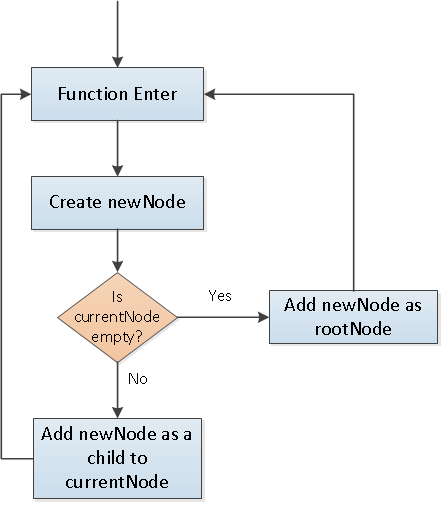
\includegraphics[width=6cm, height=6cm]{approach1.png}
  \caption{Approach Entry Point}
  \label{fig:approach1}
\end{figure}

Listing~\ref{l:treeNode} shows the data structure of each node where each \enquote{node} represents a function and in it a \enquote{\textit{name}} stores the actual name of the function. \enquote{\textit{parent}} contains the parent node of each node, and \enquote{\textit{children}} points to all the children nodes of a given node. \enquote{\textit{funcBody}} contains the actual function body of the node which is later used in the analysis to determine recursive function calls (Section~\ref{subsec:recursive}). \enquote{\textit{variables}} is an array of objects where each object contains the variable name, its type i.e. declare, read or write and a flag to determine if it was an argument or not. \enquote{\textit{isHoistableWithParent}} is a boolean flag which is set to true if Rule - 1 of hoistability for a given node is satisfied. \enquote{iid} contains the line number of the function in the source code. Lastly, \enquote{\textit{nonHoistableParents}} is an array of all the parent nodes under which the given node cannot be hoisted due to function definition conflicts (Rule-2). \par



Figure~\ref{fig:approach1}, is a flowchart diagram of the entry point of our analysis. So when a function is called, the FunctionEnter() callback is invoked in which we create a new node for the function being called. After creating the node, the analysis checks whether the \enquote{currentNode}, which is the node representing any function called previously, is empty or not. If it is empty then it is assumed that this is the very first function call of the code base and hence, the newNode is to be added as the \enquote{rootNode} of the analysis tree. On the other hand, if the currentNode is not empty, then the analysis would rightly detect a function nesting and would add the newNode as a child node to the currentNode. In both cases, the currentNode is updated at the end to newNode.\par

Next read(), write() and declare() callbacks are invoked after the functionEnter() callback finishes. These callbacks are used to check for all the parameters and variables declared or used by the function (currentNode) and then add them to the array of \enquote{variables} shown in Listing~\ref{l:treeNode}. Lastly, \enquote{instrumentCodePre()} is used to know if an eval() is direct or indirect and \enquote{literal()}is used to determine the name of the function in case of of an indirect eval(). 

\begin{figure}[H]
  \centering
  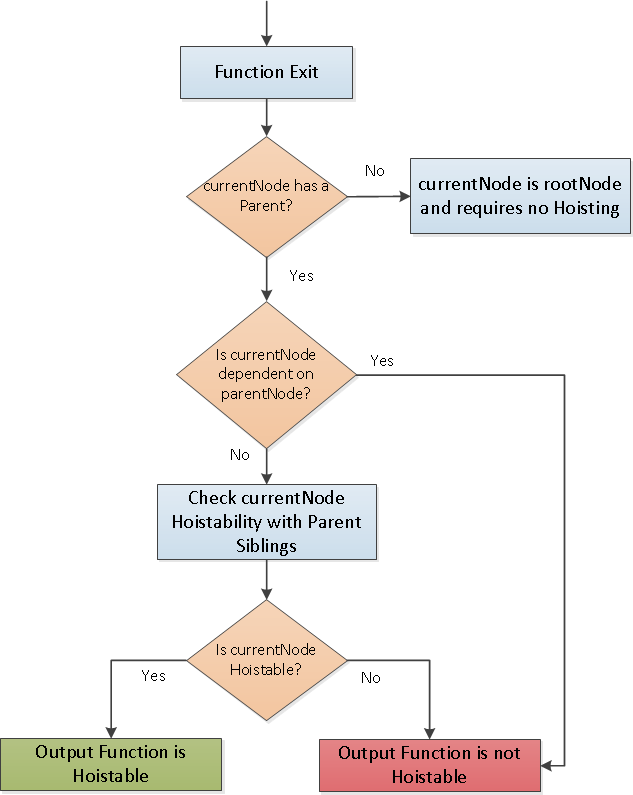
\includegraphics[width=7cm, height=7cm]{approach2.png}
  \caption{Approach Exit Point}
  \label{fig:approach2}
\end{figure}

This is how the whole tree structure is built for all the functions by the analysis. Now, when a function represented by \enquote{currentNode} in Figure~\ref{fig:approach2} exits then the functionExit() callback is invoked. In which case the analysis first checks Rule-1 (Section~\ref{sec:hoisting_rules}) of hoistability for the function (currentNode). This means that the analysis checks whether currentNode is using any of the variables or parameters defined or used by its parentNode. If yes, then the flag \enquote{isHoistableWithParent} is set to \textit{false} and at the end, this function would be marked as \enquote{Not hoistable}.\par
On the other hand, if the function (currentNode) is not dependent on its parent function (parentNode) then this flag \enquote{isHoistableWithParent} is set to \textit{true}. Now comes the second rule of hoistability (Section~\ref{sec:hoisting_rules}) which is to make sure that the scope in which the function (currentNode) is to be hoisted does not already have a function with the same definition. To verify this rule for a given function referred as currentNode in Listing~\ref{l:pseudocode} and Figure~\ref{fig:approach2}, this analysis recursively traverses through the whole tree hierarchy above the currentNode and adds all the parents which violate this rule to the list of \enquote{nonHoistableParents} of the currentNode. Thus, in the end, the analysis would output exactly under which parent the currentNode would face a definition conflict problem.

\lstset{numbers=left, numberstyle=\tiny, stepnumber=1, numbersep=5pt}
\lstset{basicstyle=\ttfamily}
\lstset{frame=tb, frame=bottomline}

\begin{lstlisting}[float,caption= Pseudocode of the Analysis ,label=l:pseudocode,language=JavaScript]
functionEnter(functionObject){

  TreeNode newNode = 
  new TreeNode(functionObject,currentNode)
  if(currentNode==null){
		tree.push(newNode)
  }
  else{
  	currentNode.addChild(newNode)
  }
   currentNode = newNode
}

functionExit(){

  checkHoistabilityWithParent(currentNode)
  if (currentNode!=null && 
  currentNode.parent!=null){
	currentNode=currentNode.parent
  }
  else if(currentNode.parent==null){
     checkHoistabilityWithParentSiblings(currentNode)
  }
}
\end{lstlisting} 

\section{Completeness of the Approach}
\label{sec:completeness}
The above mentioned approach works fine for the function declarations. In the below subsections, we are checking the coverage of our approach in different use/corner cases:

\subsection{Function Expressions}
When a function definition is assigned to a variable, it is called a \textit{function expression}. The function assigned to the variable can have a name or it can be \enquote{anonymous}, i.e. without a function name. \par

\lstset{numbers=left, numberstyle=\tiny, stepnumber=1, numbersep=5pt}
\lstset{basicstyle=\ttfamily}
\lstset{frame=tb, frame=bottomline}

\begin{lstlisting}[float,caption=Function Expression ,label=l:named_funcExp,language=JavaScript]
var one = function functionOne(param) {
  var b=1;
  var two= function functionTwo(){
     var v = param +1;
     var three = function functionThree(){
            var c = c + 1;
            return c;
          }
          return three()
      }
  return two();
}
one(2);
\end{lstlisting} 

For a given code such as in Listing~\ref{l:named_funcExp} with function expressions, we first check if the nested function expression is following hoistability Rule-1. If it is, then it is marked as hoistable and can be assigned to a new variable in the outer scope. For example, in Listing~\ref{l:named_funcExp}, where functionTwo() and functionThree() are nested inside functionOne() and  functionTwo() respectively. Our approach will first apply Rule-1 on all the functions, functionTwo() is not hoistable because it uses the local variable \enquote{param} of its parent functionOne(). FunctionThree() is marked as hoistable by our analysis because it is not using any local variables of functionTwo() and then our analysis will check hoistability Rule-2 for this function and identify any function definition or variable name conflicts with the parent function. 

In case of anonymous functions, which are basically function expression without any function names, our approach stores the function name as \enquote{anonymous} while \enquote{creating a new node} shown in Figure~\ref{fig:approach1}. For the rest of the steps, anonymous functions are treated as normal function expressions by our analysis. Figure~\ref{fig:result_func_exp} shows the our analysis output for Listing~\ref{l:named_funcExp}.


\begin{figure}[H]
  \centering
  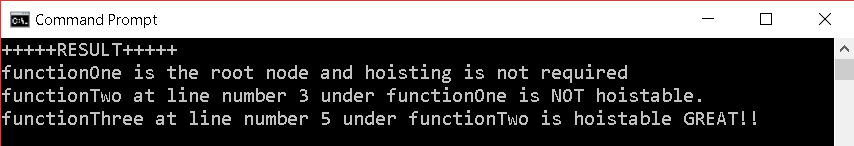
\includegraphics[width=\linewidth]{result_func_exp.png}
  \caption{Analysis Output for Listing~\ref{l:named_funcExp}}
  \label{fig:result_func_exp}
\end{figure}


\subsection{Recursive Functions}
\label{subsec:recursive}
While adding a child to a node, we compare the name and function body of the parent function with the child function. If they match and the names are not \enquote{anonymous}, then we mark the function as \textit{recursive} and we do not add it as a child function to our Tree structure again. In this way, the recursive function is only added to our Tree structure once. \par

\begin{figure}[H]
  \centering
  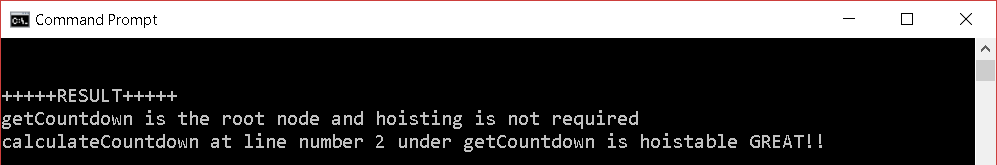
\includegraphics[width=\linewidth]{result_recursive.png}
  \caption{Analysis Output for Listing~\ref{l:recursive}}
  \label{fig:result_recursive}
\end{figure}


Consider Listing~\ref{l:recursive}, this piece of code just counts down from the given input. Here if we print the output, it should give us the value 5,4,3,2,1. Function calculateCountdown() is nested inside getCountdown() function and it is not using any local variables of the parent function. So our approach will only add calculateCountDown() as a child node to the getCountDown() function once, and then later upon functionExit() will check both hoistability Rule-1 and Rule-2 and correctly mark it as hoistable. Figure~\ref{fig:result_recursive} shows our analysis's out for Listing~\ref{l:recursive}.

\lstset{numbers=left, numberstyle=\tiny, stepnumber=1, numbersep=5pt}
\lstset{basicstyle=\ttfamily}
\lstset{frame=tb, frame=bottomline}

\begin{lstlisting}[float,caption=Recursive Functions ,label=l:recursive,language=JavaScript]
function getCountdown(countdownValue){
 function calculateCountdown(value) {
   if(value>0) {
     return calculateCountdown(value-1);
   } 
   else{
     return value;
   }
 }
    calculateCountdown(countdownValue);
}
getCountdown(5);

\end{lstlisting} 


\subsection{Direct and Indirect eval()}
A javascript program can have a function defined inside eval(). Our approach takes care of this case as well. \textit{eval()} takes the scope where it is invoked. If the function is invoked inside an eval(), then it takes the scope where it was invoked. Our approach applies Rule-1 and Rule-2 to check the hoistability of a function inside an eval().\par

In Listing~\ref{l:directEval}, directEval() is in the scope of funcEval(). So it uses the variables \enquote{x} and \enquote{y} of funcEval() and gives the output 6.  directEval() cannot be hoisted according to the hoistability Rule-1 and our analysis shows the same output as well.

\lstset{numbers=left, numberstyle=\tiny, stepnumber=1, numbersep=5pt}
\lstset{basicstyle=\ttfamily}
\lstset{frame=tb, frame=bottomline}

\begin{lstlisting}[float,caption=Direct eval() ,label=l:directEval,language=JavaScript]
x = 3;
y = 5;
function funcEval() {
 var x = 2;
 var y = 4;
 eval('function directEval() { return x + y; }');
 return directEval();
}
funcEval();
\end{lstlisting}

Now when an eval() is assigned to a variable, it is called an \textit{indirect eval}. The scope of an indirect eval() always takes the global scope no matter where is it invoked. So a function invoked using an indirect eval() is always hoistable even if it is invoked inside another function's scope.\par

In Listing~\ref{l:indirecEval}, \enquote{geval} is the reference for eval and it is invoking a function at line 7. Though indirectEval() at line 8 appears to be nested inside funcEval(), but it will not use any variables of this scope i.e. \enquote{x} or \enquote{y} at line 5 and 6 respectively. Instead it will use the global variables \enquote{x} and \enquote{y} at line 1 and line 2 for calculating the return value and will return 8. Our analysis handles this case by first detecting the presence of an indirect eval during the instrumentCodePre() and literal() jalangi2 callbacks. We store the function names in an array. In Listing~\ref{l:indirecEval}, we store inDirectEval(). While creating a child node, we do not include inDirectEval() to the current node's children. But we display it in the result that since inDirectEval() is indirect eval, it does not require hoisting. 

\lstset{numbers=left, numberstyle=\tiny, stepnumber=1, numbersep=5pt}
\lstset{basicstyle=\ttfamily}
\lstset{frame=tb, frame=bottomline}

\begin{lstlisting}[float,caption=InDirect eval() ,label=l:indirecEval,language=JavaScript]
x = 3;
y = 5;
var geval = eval;
function funcEval() {
  var x = 2;
  var y = 4;
  geval('function indirectEval() { return x + y; }');
  return indirectEval();
}
funcEval();
\end{lstlisting}

In cases where the functions defined inside direct or indirect eval() are nested, our approach successfully handles the hoistability detection by treating those functions as normal functions declarations or expressions only with different scopes.

\section{Evaluation and Results}
\label{sec:evaluation}

In order to evaluate the accuracy our analysis, it was first executed on smaller but complicated Javascript programs like the ones shown in Listings~\ref{l:indirecEval},~\ref{l:directEval},~\ref{l:named_funcExp},~\ref{l:recursive}. The analysis was able to successfully detect all hoistable functions by checking both Rule-1 and Rule-2 on such examples. \par For example, Figure~\ref{fig:output} is the screen shot of the output our analysis gave when we executed it on the code given in Listing~\ref{l:nestedFunction}.

\begin{figure}[H]
  \centering
  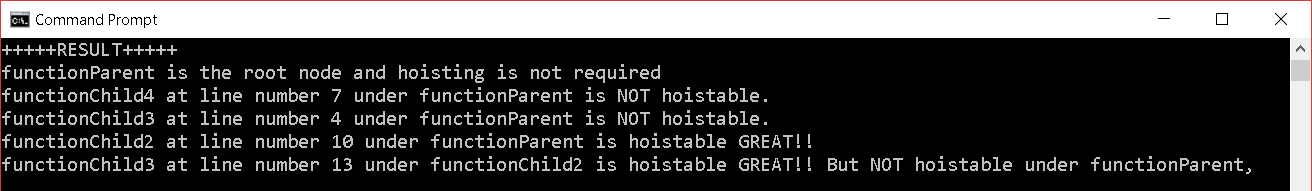
\includegraphics[width=\linewidth]{result.png}
  \caption{Analysis Output for Listing~\ref{l:nestedFunction}}
  \label{fig:output}
\end{figure}


Next phase of the evaluation was focused on detecting any difference in execution time of a code base with hoisted functions and without any hoisting. To do this a famous Javascript library \enquote{Lodash} was selected and following steps were performed:


\begin{enumerate}
  \item First, the provided test suit of the Lodash library was executed on the original version of the repository multiple times and an average execution time was noted down.
  \item Then the analysis was executed on the same repository which marked all the hoistable and non-hoistable functions.  
  \item Then as per the analysis results, manual hoisting of the repository was performed.
  \item In the end, the Lodash test suit was again executed multiple times but this time on the updated hoisted version of the repository and an average execution time of the test suite was noted down.
  \end{enumerate}

Following are the results which were obtained:
\begin{table}[h!]
  \begin{center}
    \caption{}
    \label{tab:evaluation}
    \begin{tabular}{l|c|r|} % <-- Alignments: 1st column left, 2nd middle and 3rd right, with vertical lines in between
      \textbf{Library} & \multicolumn{2}{c|}{\textbf{Avg. Execution Time}}\\
      \textbf{} & \textbf{Original Repository} & \textbf{Hoisted Repository}\\
      \hline
      Lodash & 9767ms & 9704ms\\
    \end{tabular}
  \end{center}
\end{table}


So it can be seen from the results in Table 1, that after only hoisting 7 functions an improvement of around 63ms was observed in the execution time.

\section{Limitations and Future Work}
\label{sec:limitation}
Our approach has few limitations which can be used for future work. Firstly, while checking recursive functions, we just compare the names and function body of the parent function with the child function. But in practice, Javascript allows for nested functions to have the same same name and function body as its parent function, in such a case our approach would detect that as a recursive function as well which would be incorrect. \par

Secondly, if there is a nested function which is not dependent on any of its parent variables or parameters and has no function definition conflicts with its parent's siblings but calls a function defined in the same scope as itself. For such a program our approach just checks the two rules of hoistability and would mark it as hoistable even though when hoisted, this function would throw an exception as it was calling a function inside it which is no longer accessible in its new hoisted scope. This is something that can be improved in future. \par

Moreover, our analysis tells exactly under which parent a function can't be hoisted but it does not tell under which parent hoisting the function would be most optimal. Such kind of information can be helpful in the case where there are multiple options of hoistability for a particular function and hoisting the function at one place might give better performance than the other. Plus, in case of indirect eval, our anaylsis is unable to detect hoistability of any nested functions defined inside of the indirect eval itself. 



\section{Conclusion}
\label{sec:conclusion}
Nested functions have to be avoided when it does not serve the purpose of abstraction and encapsulation of data. Also, nesting functions reduces the performance. So it is better to identify such functions and hoist them. Our approach uses two basic rules of hoistability to identify if a function can be hoisted or not and except for some limitations described in Section~\ref{sec:limitation} we are successful in identifying functions which can be hoisted. Also, evaluation of approach on javascript libraries like Lodash showed positive results by showing improvements in execution time.\par

\bibliographystyle{abbrv}
\begin{thebibliography}{1}
\softraggedright


\bibitem [K. Sen, S. Kalasapur, T. Brutch, and S. Gibbs]
K. Sen, S. Kalasapur, T. Brutch, and S. Gibbs. Jalangi: A selective
record-replay and dynamic analysis framework for JavaScript. In Proceedings of the 2013 9th
Joint Meeting on Foundations of Software Engineering, pages 488–498. ACM, 2013.

%\bibitem [samsung]
%Samsung. Jalangi2: Dynamic analysis framework for JavaScript. URL
%https://github.com/Samsung/jalangi2.

%\bibitem  [nodejs]
%nodejs
%https://nodejs.org/
%\bibitem  [underscore]
%underscore
%https://github.com/jashkenas/underscore
%\bibitem  [q]
%q
%https://github.com/kriskowal/q
%\bibitem  [lodash]
%lodash
%https://github.com/lodash/lodash


\end{thebibliography}


\end{document}
